\documentclass[10pt]{article}

\usepackage[letterpaper]{geometry}
\usepackage{color}
\usepackage{hyperref}
\usepackage{fancyhdr}
\usepackage{sectsty}
\usepackage{amsmath}
\usepackage{graphicx}
\usepackage{pdflscape}

\setlength{\headheight}{0pt}
\setlength{\headwidth}{6.5in}
%\pagestyle{fancy}

\setlength{\textwidth}{6.5in}
\setlength{\textheight}{8.5in}
\setlength{\topmargin}{0in}
\setlength{\oddsidemargin}{0.0in}
\setlength{\evensidemargin}{0.0in}
\setlength{\rightmargin}{0.0in}
\setlength{\footskip}{.5in}
\setlength{\parindent}{0pt}

\newcommand{\angstrom}{\text{\normalfont\AA}}
\newcommand{\blankline}{\quad\pagebreak[3]}
\sectionfont{\fontsize{13}{15}\selectfont}


\linespread{1.07}

\title{\large{Conceptual Design Report} \\
        \Large{\bf Inverse Compton Scattering Extreme Ultra-Violet Light Source}}
        
\author{\large Chong Shik Park, Ph.D, \\
Korea University, Sejong 30019, South Korea}

\begin{document}

\maketitle

\tableofcontents

\newpage
\begin{landscape}
\null
\vfill
\begin{figure}[ht]
  \centering
    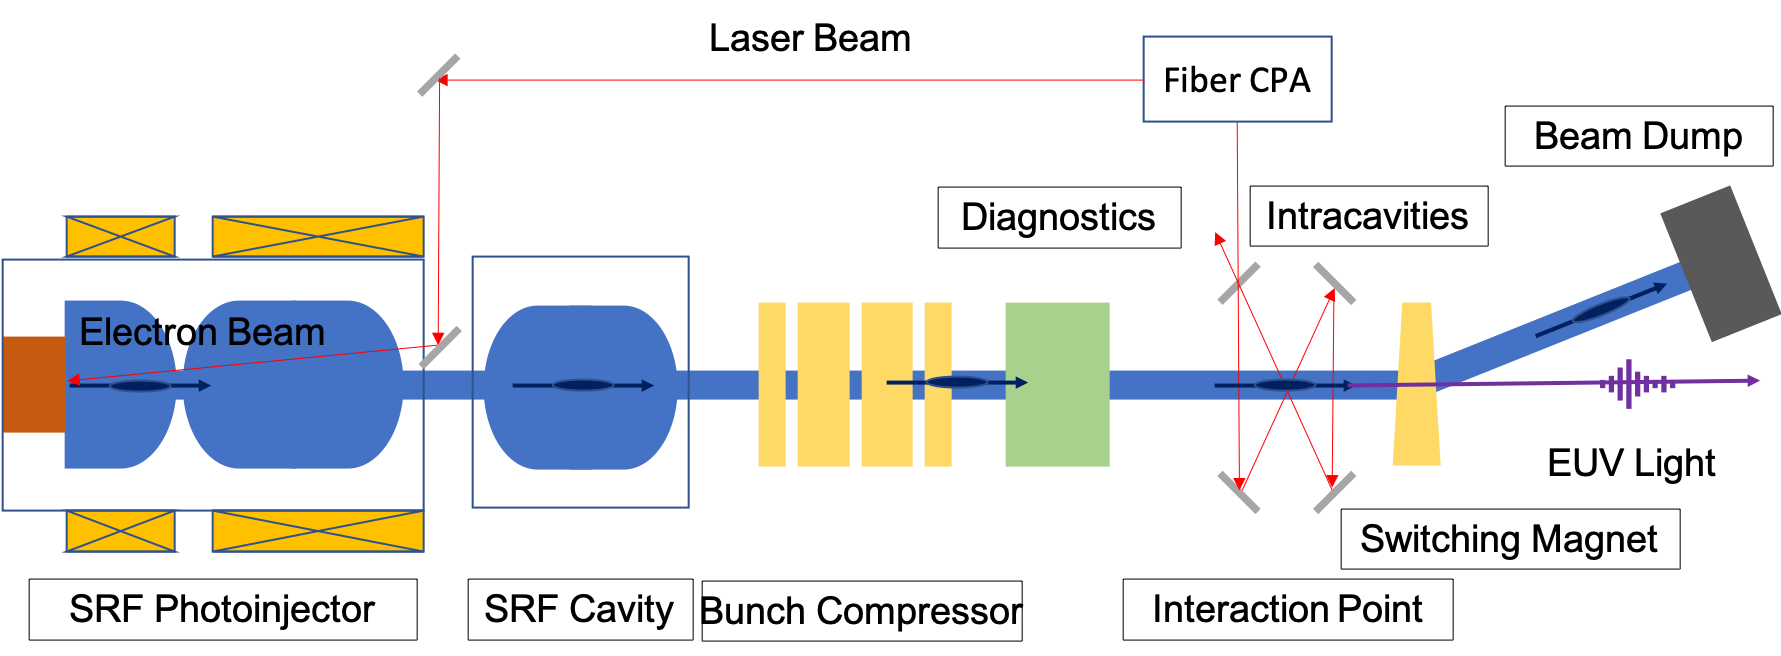
\includegraphics[width=8in]{img/ics-layout.png}
    \caption{Inverse Compton Scattering EUV Light Source Layout}
    \label{fig:layout}
\end{figure}
\vfill

\end{landscape}

\newpage

\section{Introduction}

  \subsection{EUV Light Source Design Criteria}
  
  \subsection{Accelerator-Based EUV Light Sources}
  
  \subsection{ICS EUV Light Source Design Concept and Performance Goal}


\blankline
\blankline

\section{Overview of Inverse Compton Scattering EUV Light Source}

  \subsection{Physics of Inverse Compton Scattering}
  
  \subsection{Accelerator System}
  
  \subsection{Laser System}
  
  
\blankline
\blankline
  
\section{Electron Injector - Superconducting RF Photoinjector}

  \subsection{Design Requirements}
  
  \subsection{Accelerator Physics Design}
  
  \subsection{R\&D Required}  


\blankline
\blankline

\section{Superconducting RF Linac}

  \subsection{Design Requirements}
  
  \subsection{Accelerator Physics Design}
  
  \subsection{R\&D Required}  


\blankline
\blankline

\section{Incident Laser System and Interaction Region}

  \subsection{Design Requirements}
  
  \subsection{Accelerator Physics Design}
  
  \subsection{R\&D Required}  


\blankline
\blankline

\section{System Integration and Control}

  \subsection{Design Requirements}
  
  \subsection{Accelerator Physics Design}
  
  \subsection{R\&D Required}  


\blankline
\blankline


\section{Cost Estimate}

  \subsection{Basis of Estimate}
  
  \subsection{Cost Summary}


%%%%%%%%%%%%%%%%%%%%%%%%%%%%%%%%%%%%%%%%%%%%%%%%%%%




%\begin{thebibliography}{77}
%
%  \raggedright
%
%  \bibitem{blahblah}
%  blahblah
%
%
%\end{thebibliography}

\end{document}
